\documentclass[a4paper,12pt]{article}
% Package to make citations superscrit with brackets
\usepackage[super,square]{natbib}
% Package to change margin size
\usepackage{anysize}
\marginsize{2cm}{2cm}{1cm}{2cm}
% Package to make headers
\usepackage{fancyhdr}
\renewcommand{\headrulewidth}{0pt}
% Package for highligths
\usepackage{soul}
% Colors for the references links
\usepackage[dvipsnames]{xcolor}
% Package to link references
\usepackage{hyperref}
\usepackage{graphicx}
\hypersetup{
    colorlinks=true,
    linkcolor=black,
    citecolor=CadetBlue,
    filecolor=CadetBlue,      
    urlcolor=CadetBlue,
}
% Package for lorem ipsum
\usepackage{lipsum}
% Package for multicolumn
\usepackage{multicol}
% Package for removing paragraph identations
\usepackage{parskip}
\setlength\columnsep{18pt}
% Sets bastract
\renewenvironment{abstract}
 {\par\noindent\textbf{\abstractname}\ \ignorespaces \\}
 {\par\noindent\medskip}



 
\begin{document}
% Makes header
\pagestyle{fancy}
\thispagestyle{empty}
\fancyhead[R]{\textit{EE1200}}
\fancyhead[L]{}
% Makes footnotes with an asterisk
\renewcommand*{\thefootnote}{\fnsymbol{footnote}}
\begin{center}
\Large{\textbf{Experiment 01}}
\vspace{0.4cm}
\normalsize
\\ Aditya Tripathy - ee24btech11001, Durgi Swaraj Sharma - ee24btech11018\\
\medskip
\normalsize
\end{center}
{\color{gray}\hrule}
\vspace{0.4cm}
\begin{abstract}
In Experiment-01, we produced Lissajous figures on an oscilloscope, and also captured a one time event on it.
\end{abstract}
{\color{gray}\hrule}
\medskip
\section{Part 1 - Lissajous figures}
\subsection{Objective}
To produce and verify Lissajous figures using an oscilloscope, a function generator, and Python.
\subsection{Apparatus}
\begin{itemize}
\item Oscilloscope
\item Two channel function generator
\item Connectimng wires and probes
\item A computer to verify the results on
\end{itemize}
\subsection{Theory}
Lissajous figures are complex patterns formed when two sinusoidal signals are applied to the $x$ and $y$ axis as inputs to an oscilloscope.
Their shapes are hence dependent on the many parameters that make each sinusoidal signal.
\subsection{Procedure}
\begin{enumerate}
\item Connections
\begin{itemize}
\item Connect the two channels of the oscilloscope with the channels of the function generator, using 4 cables and the oscilloscope probes.
\end{itemize}
\item Device Setup
\begin{itemize}
\item Turn the signals ON on the function generator, and set up sinusoidal outputs for both the channels.
\item Ensure that the oscilloscope reads these signals, use the auto-scale feature if necessary.
\item To change the plotting from $Y-T$ to $X-Y$, press the $Main/Delayed$ button, and in the menu, change the Time Base from $Y-T$ to $X-Y$.
\item Align Phase on the function generator to remove any inaccuracies.
\end{itemize}
\item Modify the various parameters on the function generator, Align Phase each time, and capture the Lissajous figures on the oscilloscope screen.
\end{enumerate}
The captured Lissajous figures are shown in the next segment.
\subsection{Justification}
We will be using Python and the Matplotlib and Numpy libraries to verify our experiment. The following code plots out the theoretical Lissajous figures depending on the values of Voltage amplitudes, frequencies, and phase of the two channnels.
\begin{verbatim}
import numpy as np
import matplotlib.pyplot as plt
t = np.linspace(-3, 3, 1000)
A1 = {amplitude of signal 1}
f1 = {frequency of signal 1}
phi1 = {phase of signal 1 in radians}
 x = A1 * np.sin(2 * np.pi * f1 * t + phi1 )
A2 = {amplitude of signal 2}
f2 = {frequency of signal 2}
phi2 = {phase of signal 2 in radians}
y = A2 * np.sin(2 * np.pi * f2 * t + phi2 )
plt.plot(x, y)
plt.savefig("plot1.png")
plt.show()
\end{verbatim}
By following the procediure for different values of the voltage parameters, we produced the following six Lissajous figures and verified them using the previously mentioned code.
The parameters for the signals used are present in the pictures of the function generator menu.
\subsubsection{1.}
	  \begin{center}
		  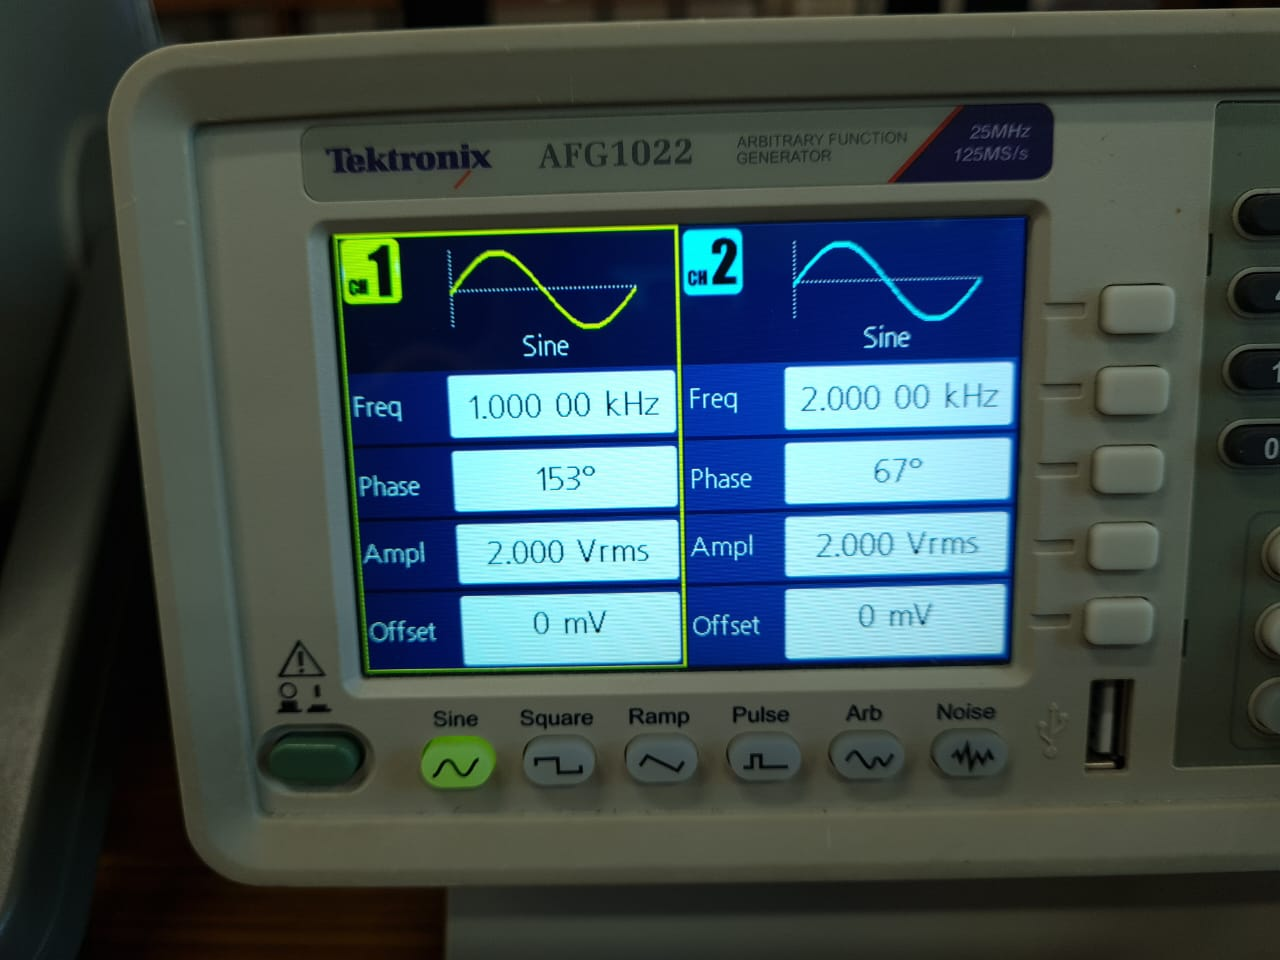
\includegraphics[width=0.5\columnwidth]{/home/gvt1/Work/ECLab2025/experiment01/figs/a2.jpg}\\
		  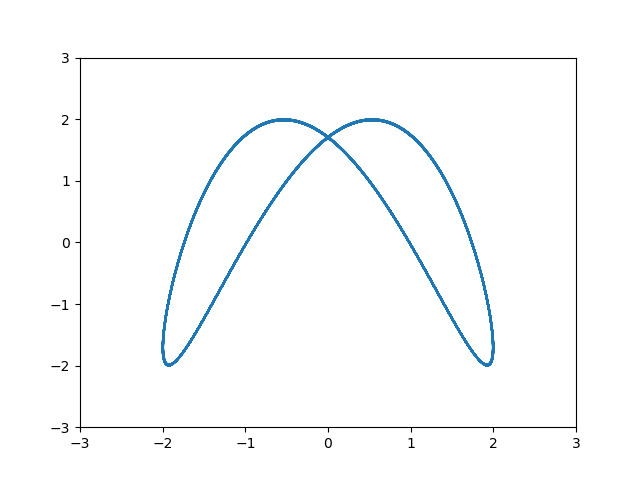
\includegraphics[width=0.4\columnwidth]{/home/gvt1/Work/ECLab2025/experiment01/figs/a.jpeg}
		  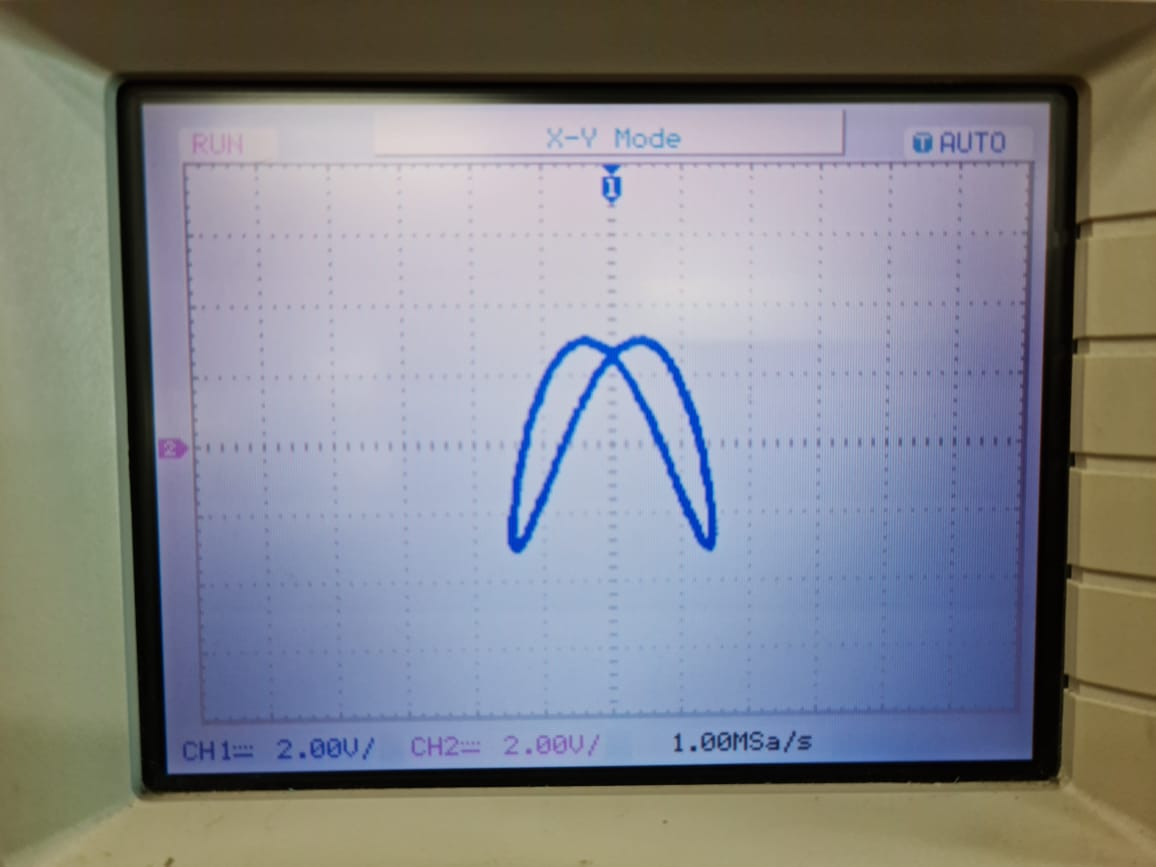
\includegraphics[width=0.4\columnwidth]{/home/gvt1/Work/ECLab2025/experiment01/figs/a1.jpg}
	  \end{center}
  \subsubsection{2.}
	  \begin{center}
		  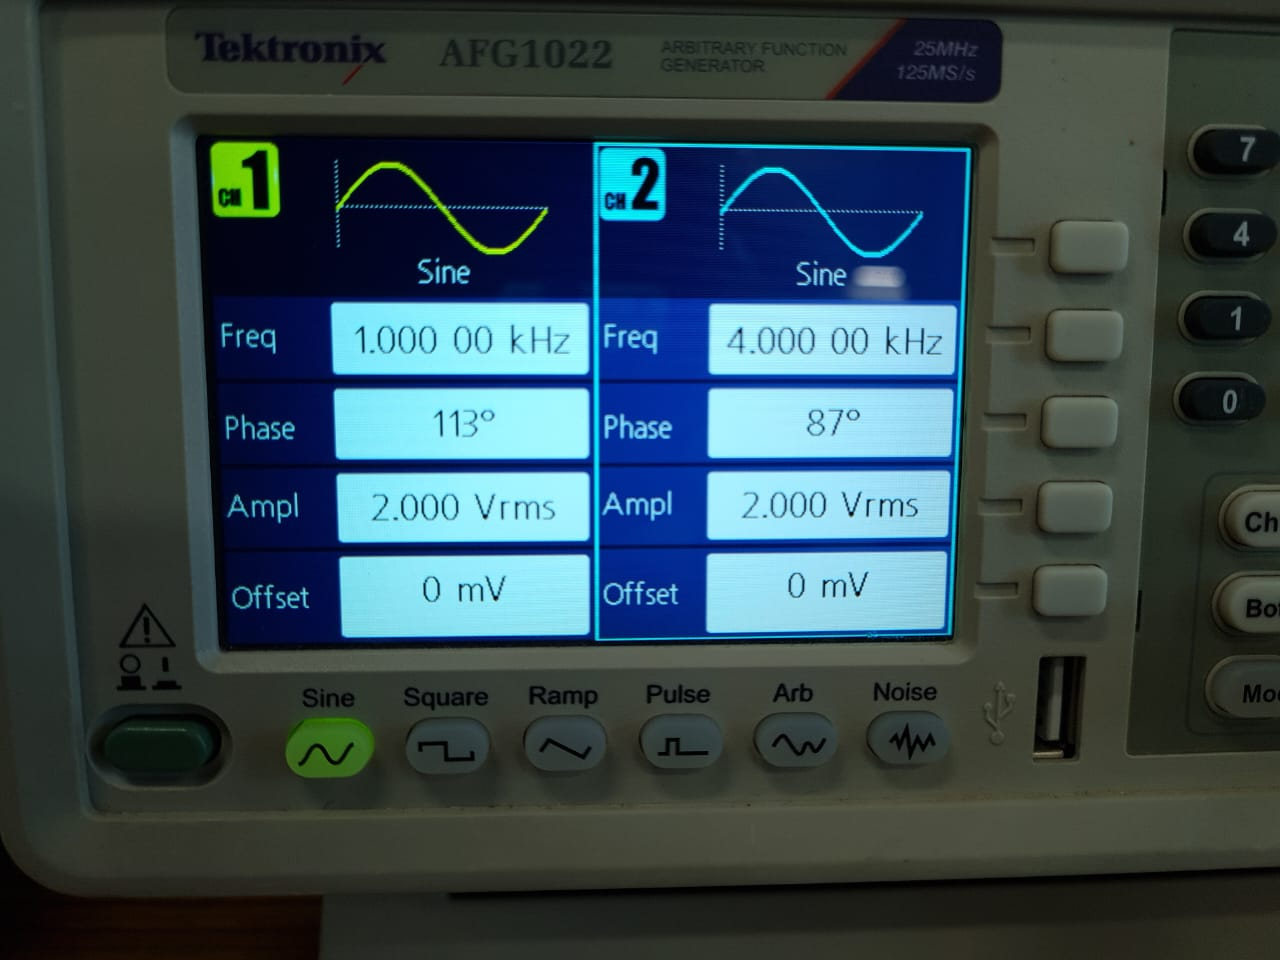
\includegraphics[width=0.5\columnwidth]{/home/gvt1/Work/ECLab2025/experiment01/figs/b2.jpg}\\
		  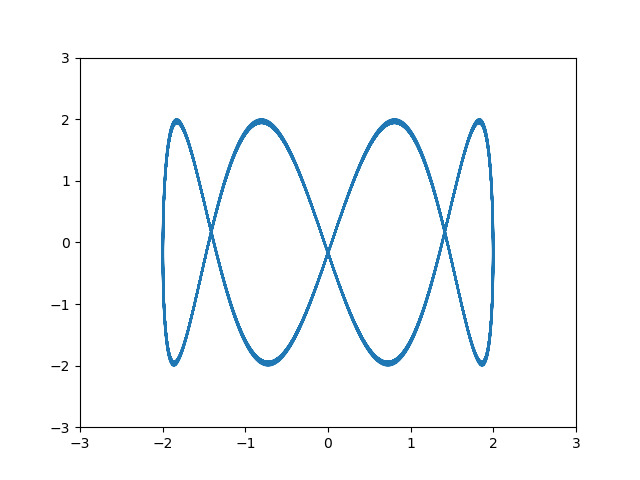
\includegraphics[width=0.4\columnwidth]{/home/gvt1/Work/ECLab2025/experiment01/figs/b.jpg}
		  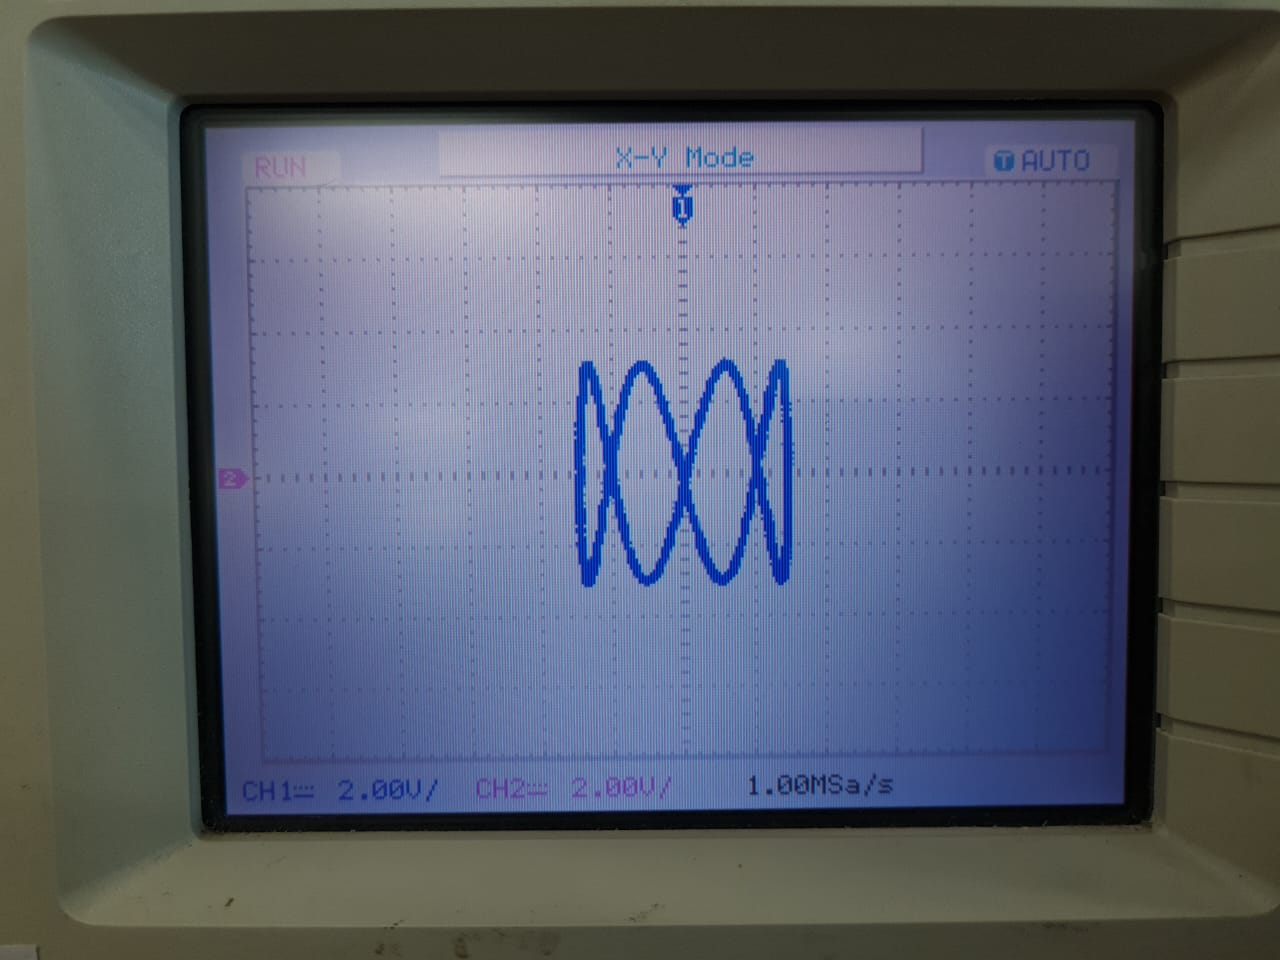
\includegraphics[width=0.4\columnwidth]{/home/gvt1/Work/ECLab2025/experiment01/figs/b1.jpg}
	  \end{center}
  \subsubsection{3.}
	  \begin{center}
		  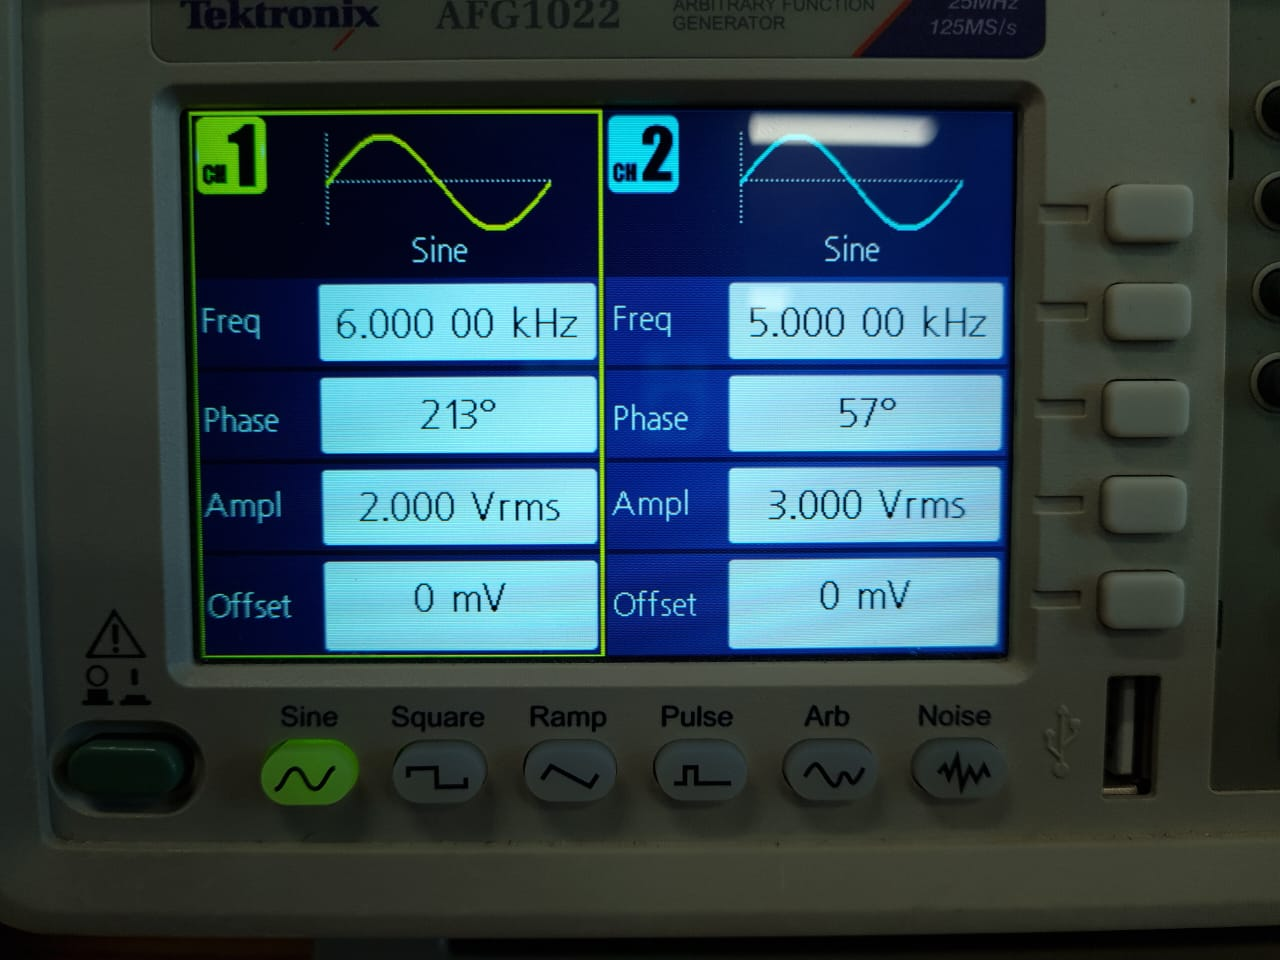
\includegraphics[width=0.5\columnwidth]{/home/gvt1/Work/ECLab2025/experiment01/figs/c2.jpg}\\
		  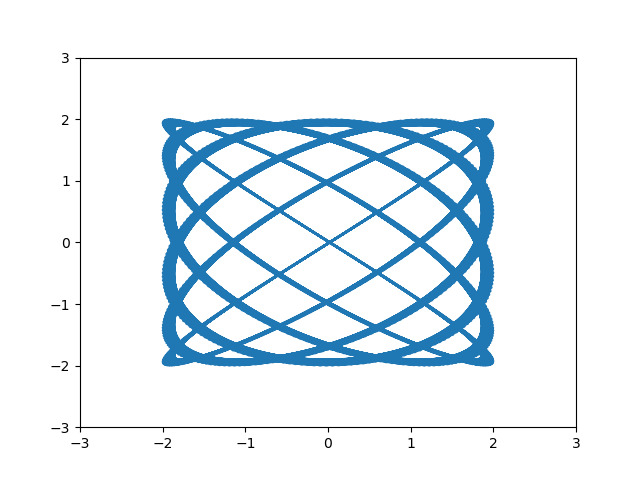
\includegraphics[width=0.4\columnwidth]{/home/gvt1/Work/ECLab2025/experiment01/figs/c.jpg}
		  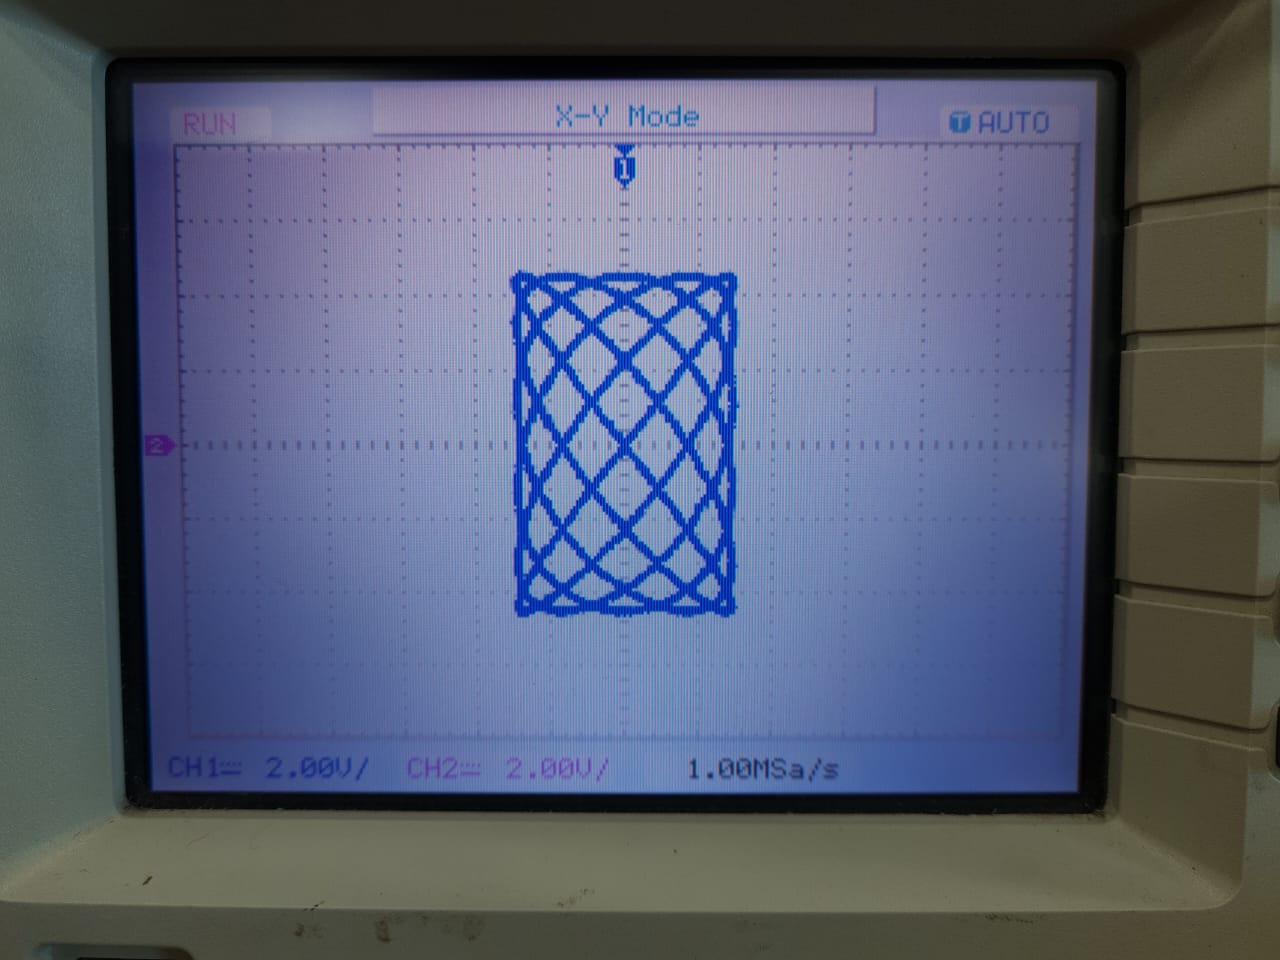
\includegraphics[width=0.4\columnwidth]{/home/gvt1/Work/ECLab2025/experiment01/figs/c1.jpg}
	  \end{center}
  \subsubsection{4.}
	  \begin{center}
		  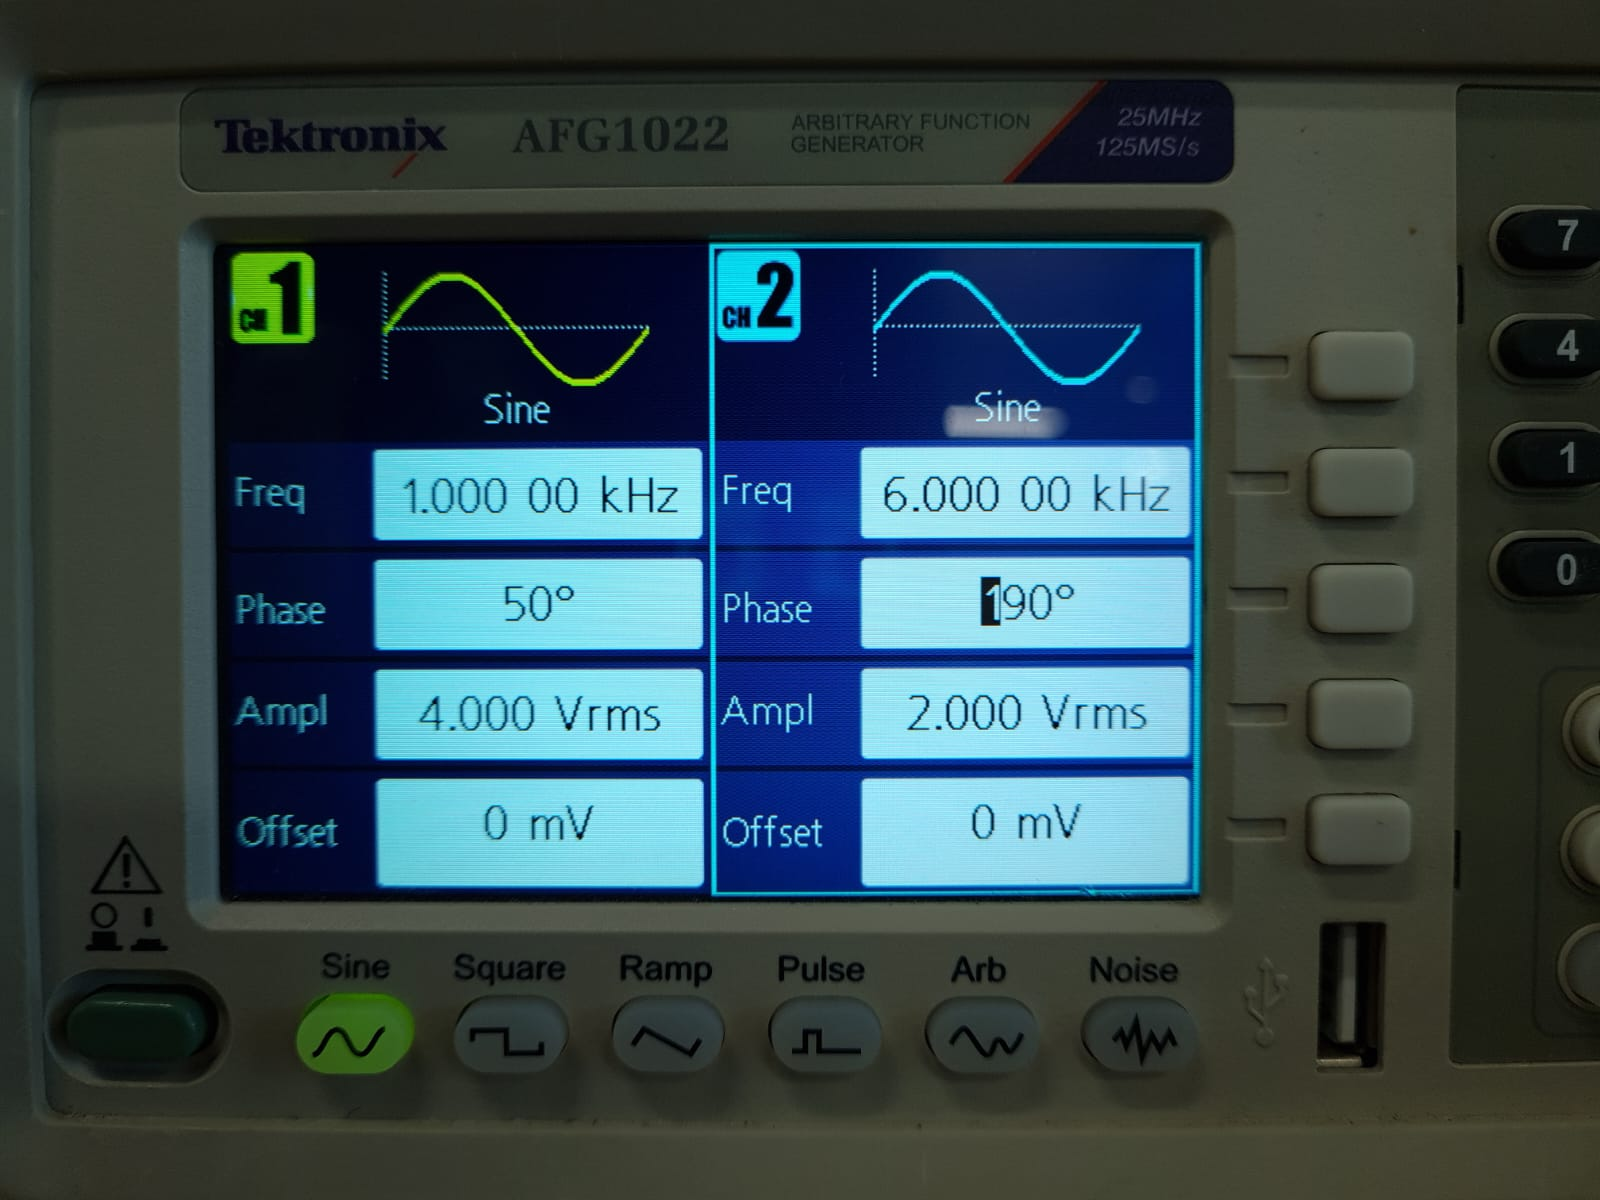
\includegraphics[width=0.5\columnwidth]{/home/gvt1/Work/ECLab2025/experiment01/figs/f2.jpg}\\
		  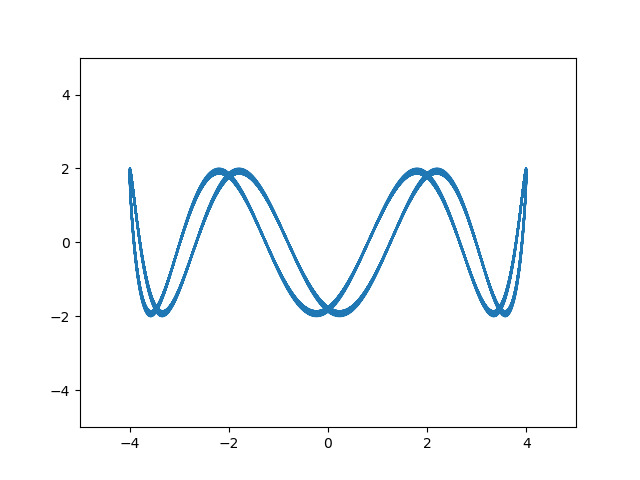
\includegraphics[width=0.4\columnwidth]{/home/gvt1/Work/ECLab2025/experiment01/figs/f.jpg}
		  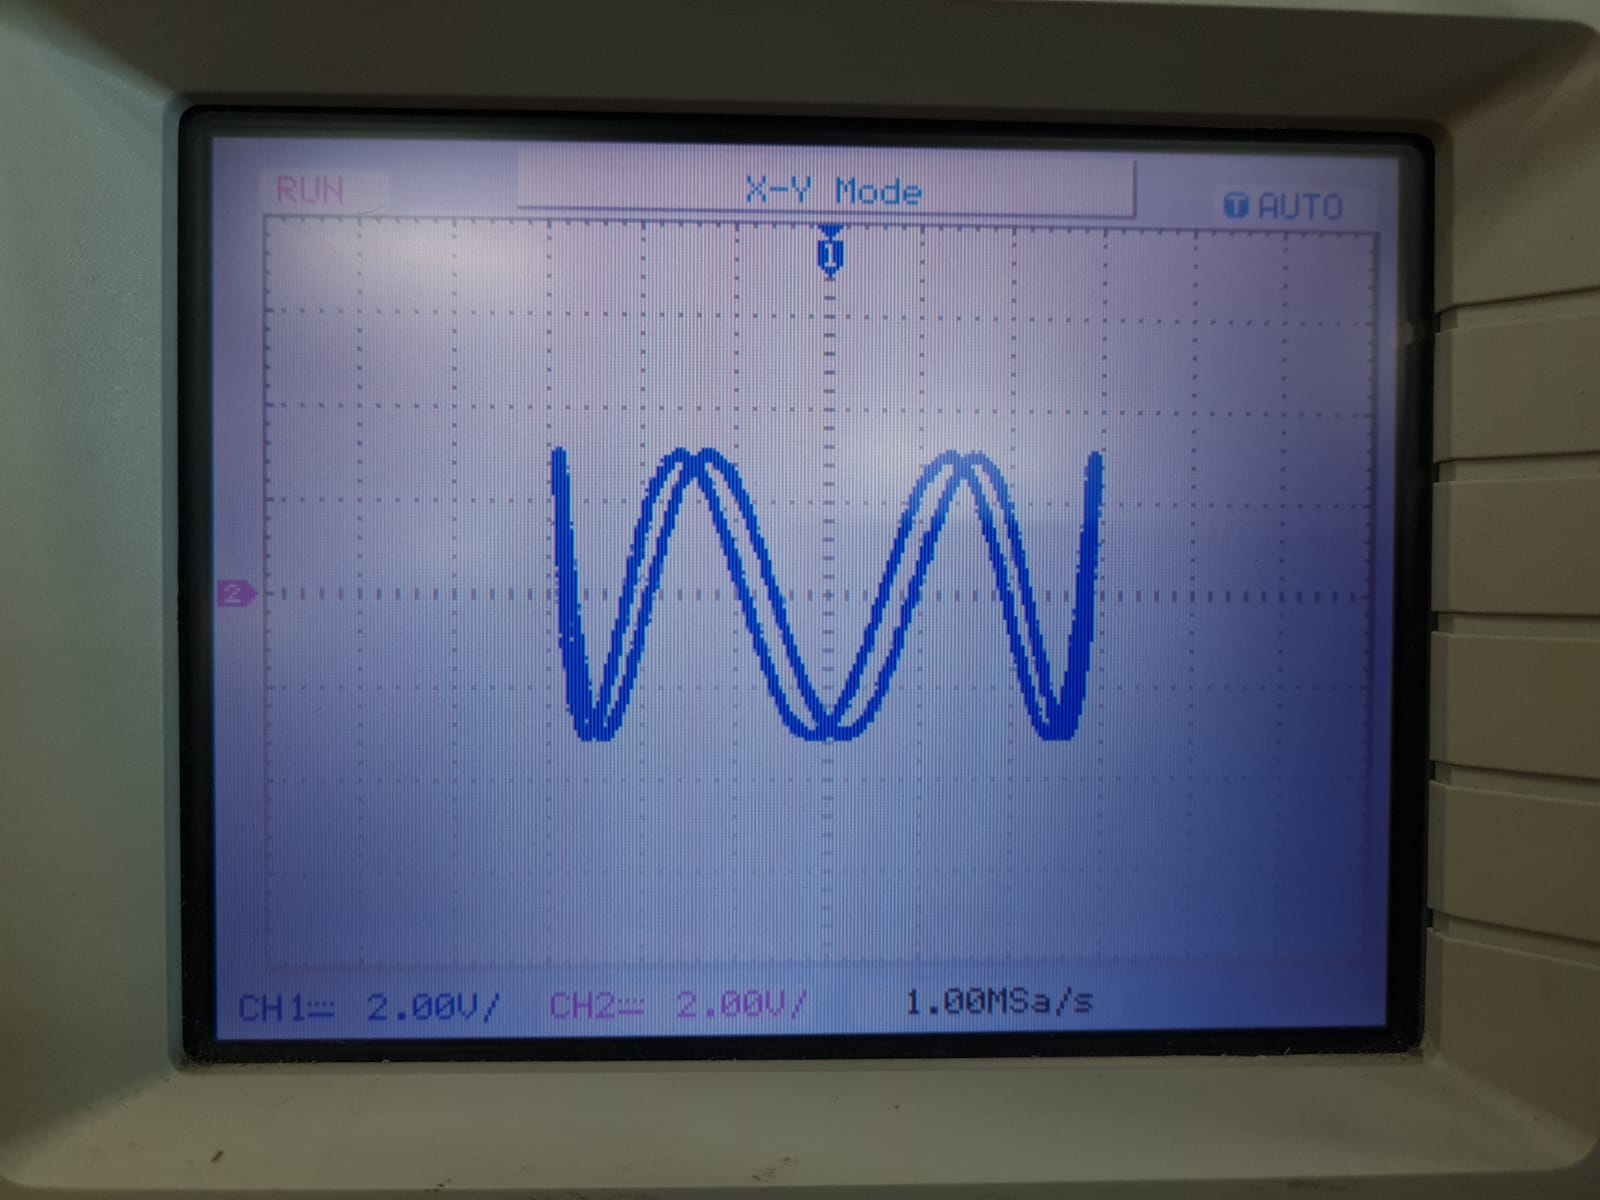
\includegraphics[width=0.4\columnwidth]{/home/gvt1/Work/ECLab2025/experiment01/figs/f1.jpg}
	  \end{center}
  \subsubsection{5.}
	  \begin{center}
		  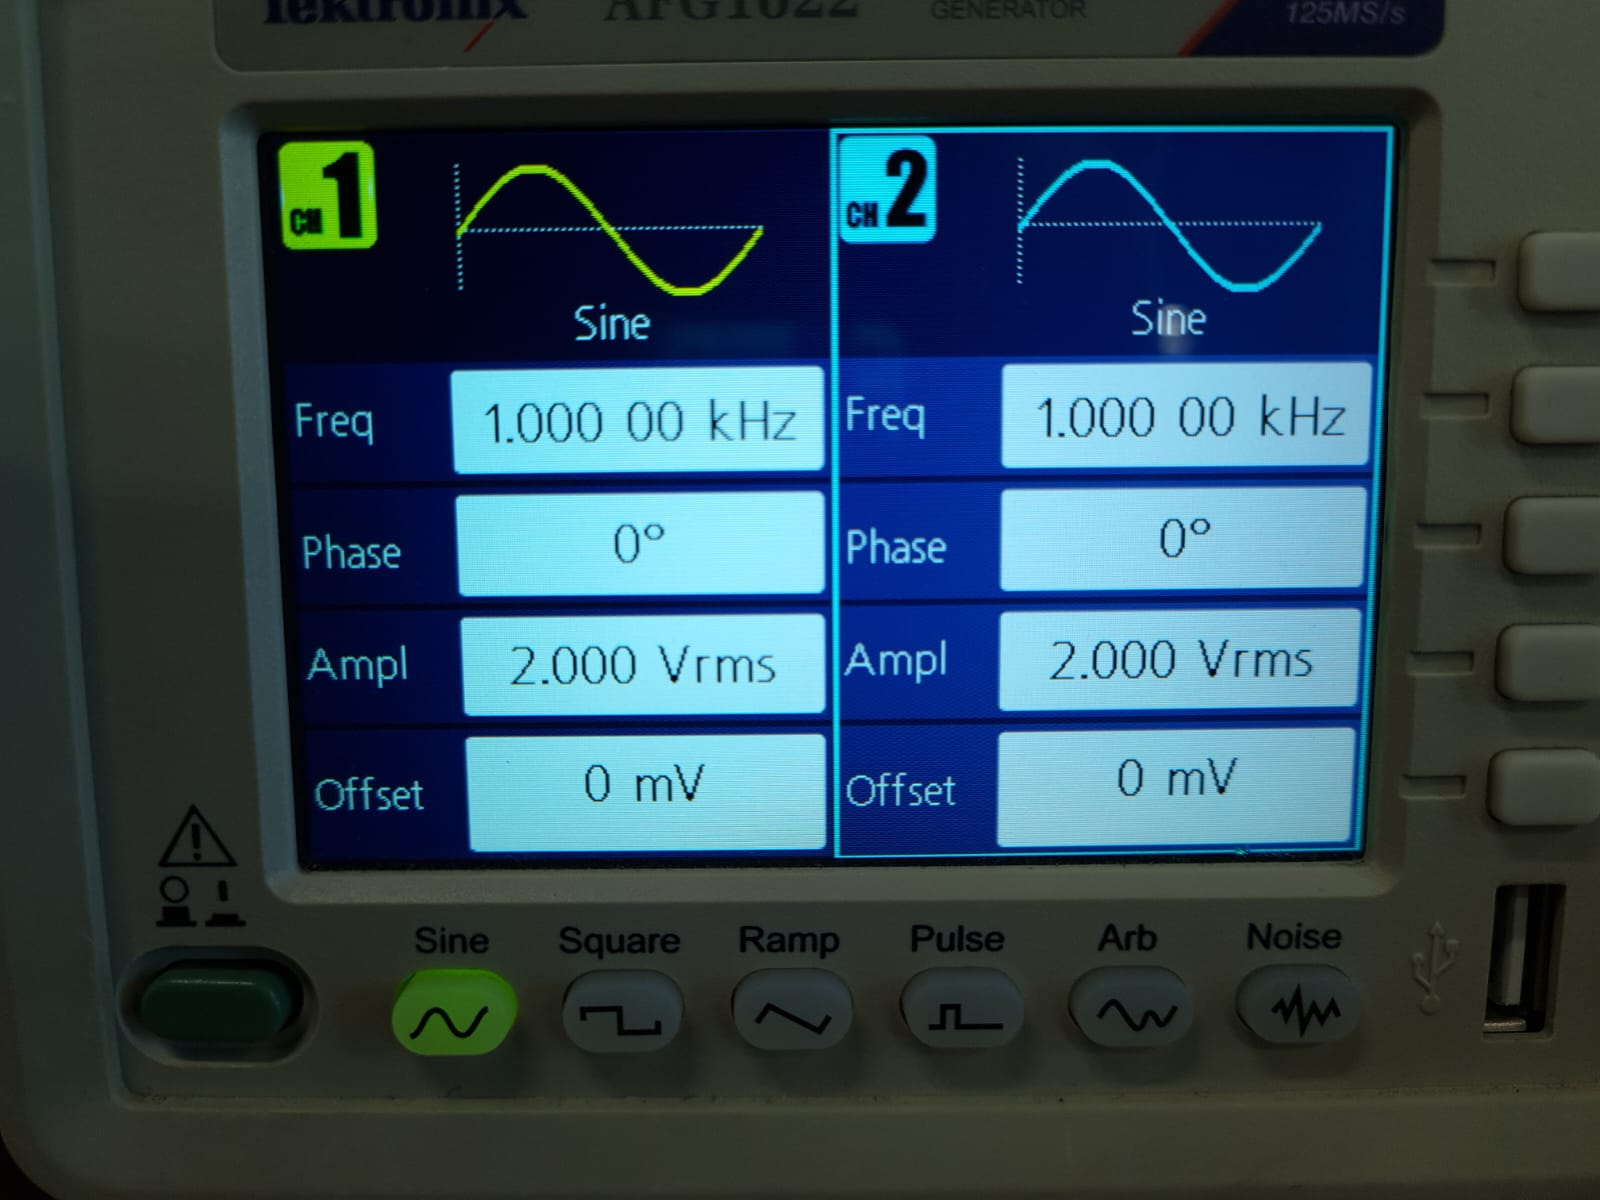
\includegraphics[width=0.5\columnwidth]{/home/gvt1/Work/ECLab2025/experiment01/figs/d2.jpg}\\
		  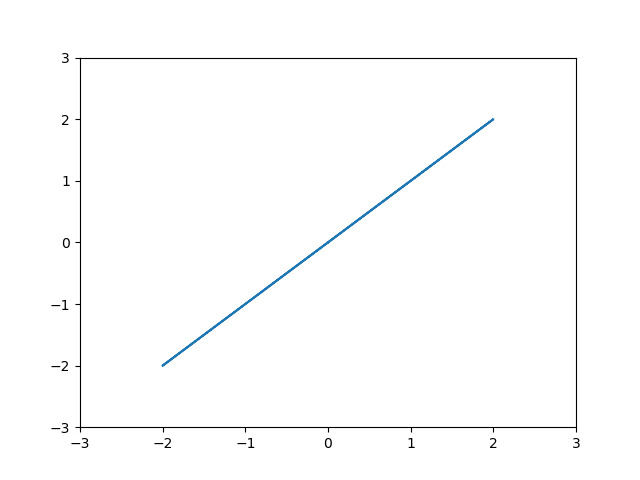
\includegraphics[width=0.4\columnwidth]{/home/gvt1/Work/ECLab2025/experiment01/figs/d.jpg}
		  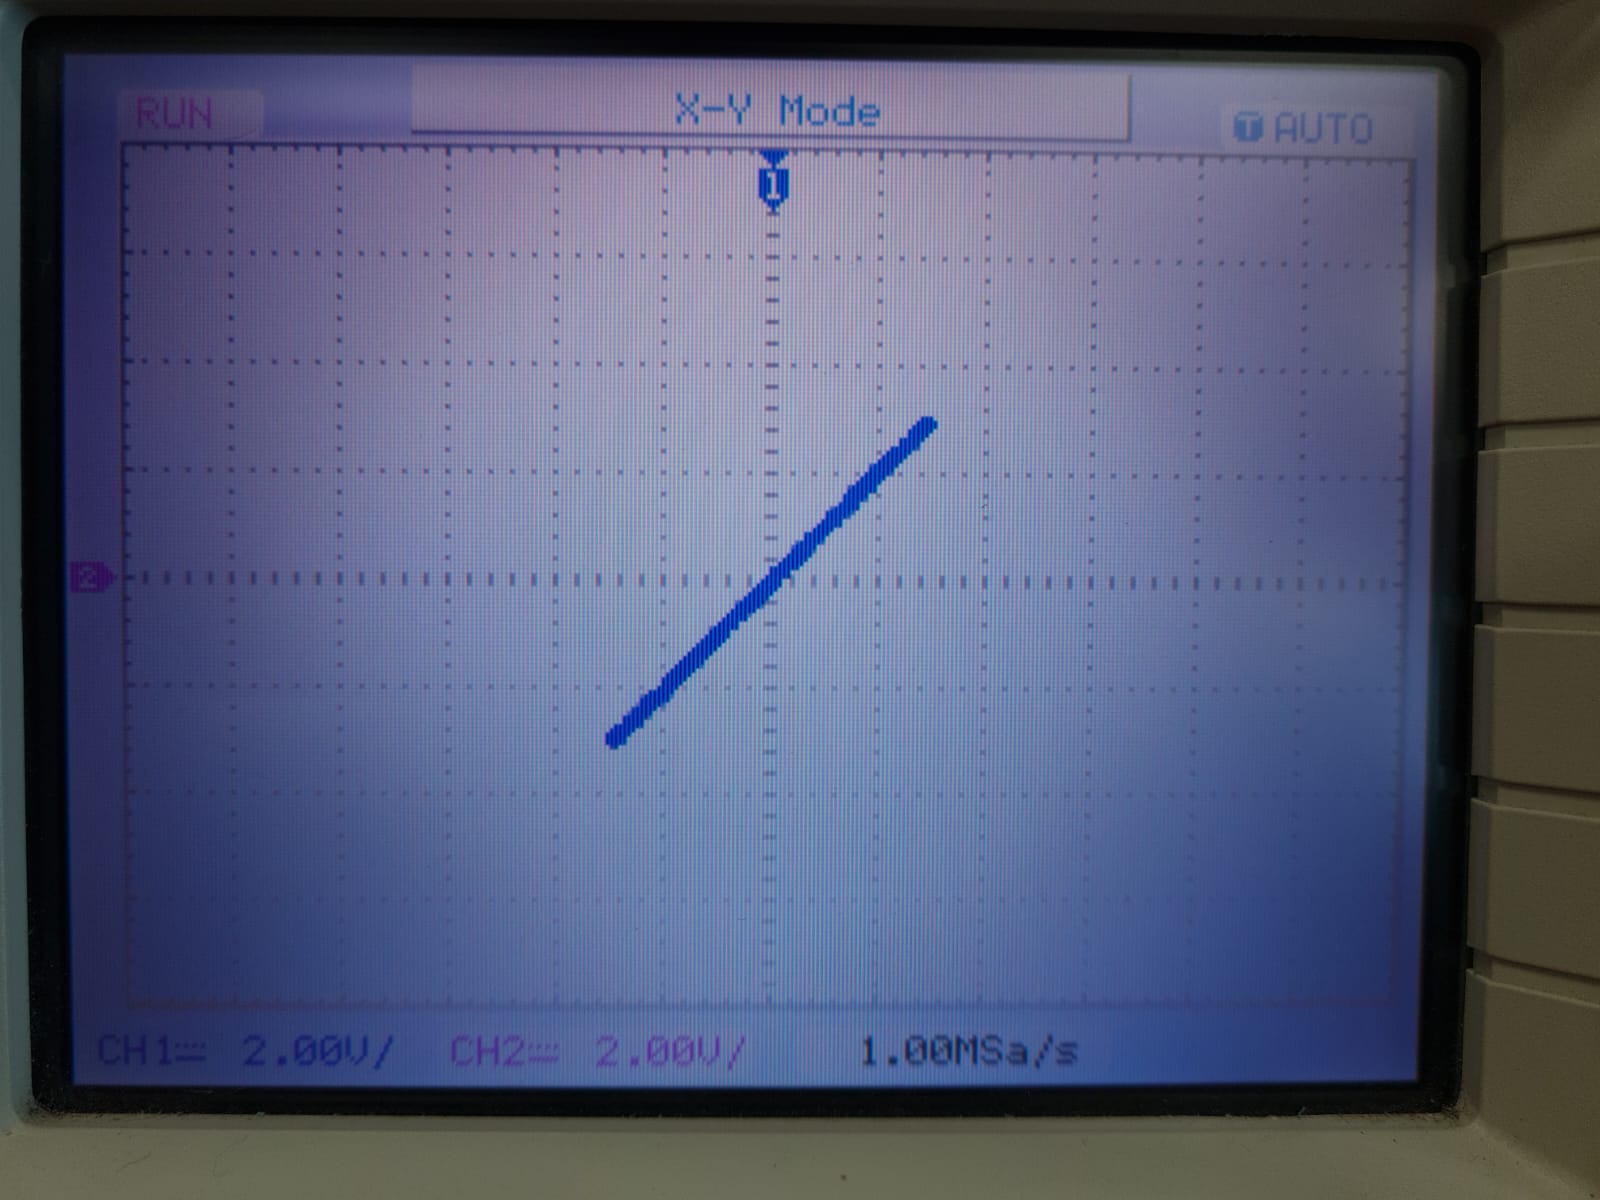
\includegraphics[width=0.4\columnwidth]{/home/gvt1/Work/ECLab2025/experiment01/figs/d1.jpg}\\
		  When all parameters for both the signals are equal, in the Lissajous figures essentially $x = y$, resulting in a straight line.
	  \end{center}
  \subsubsection{6.}
	  \begin{center}
		  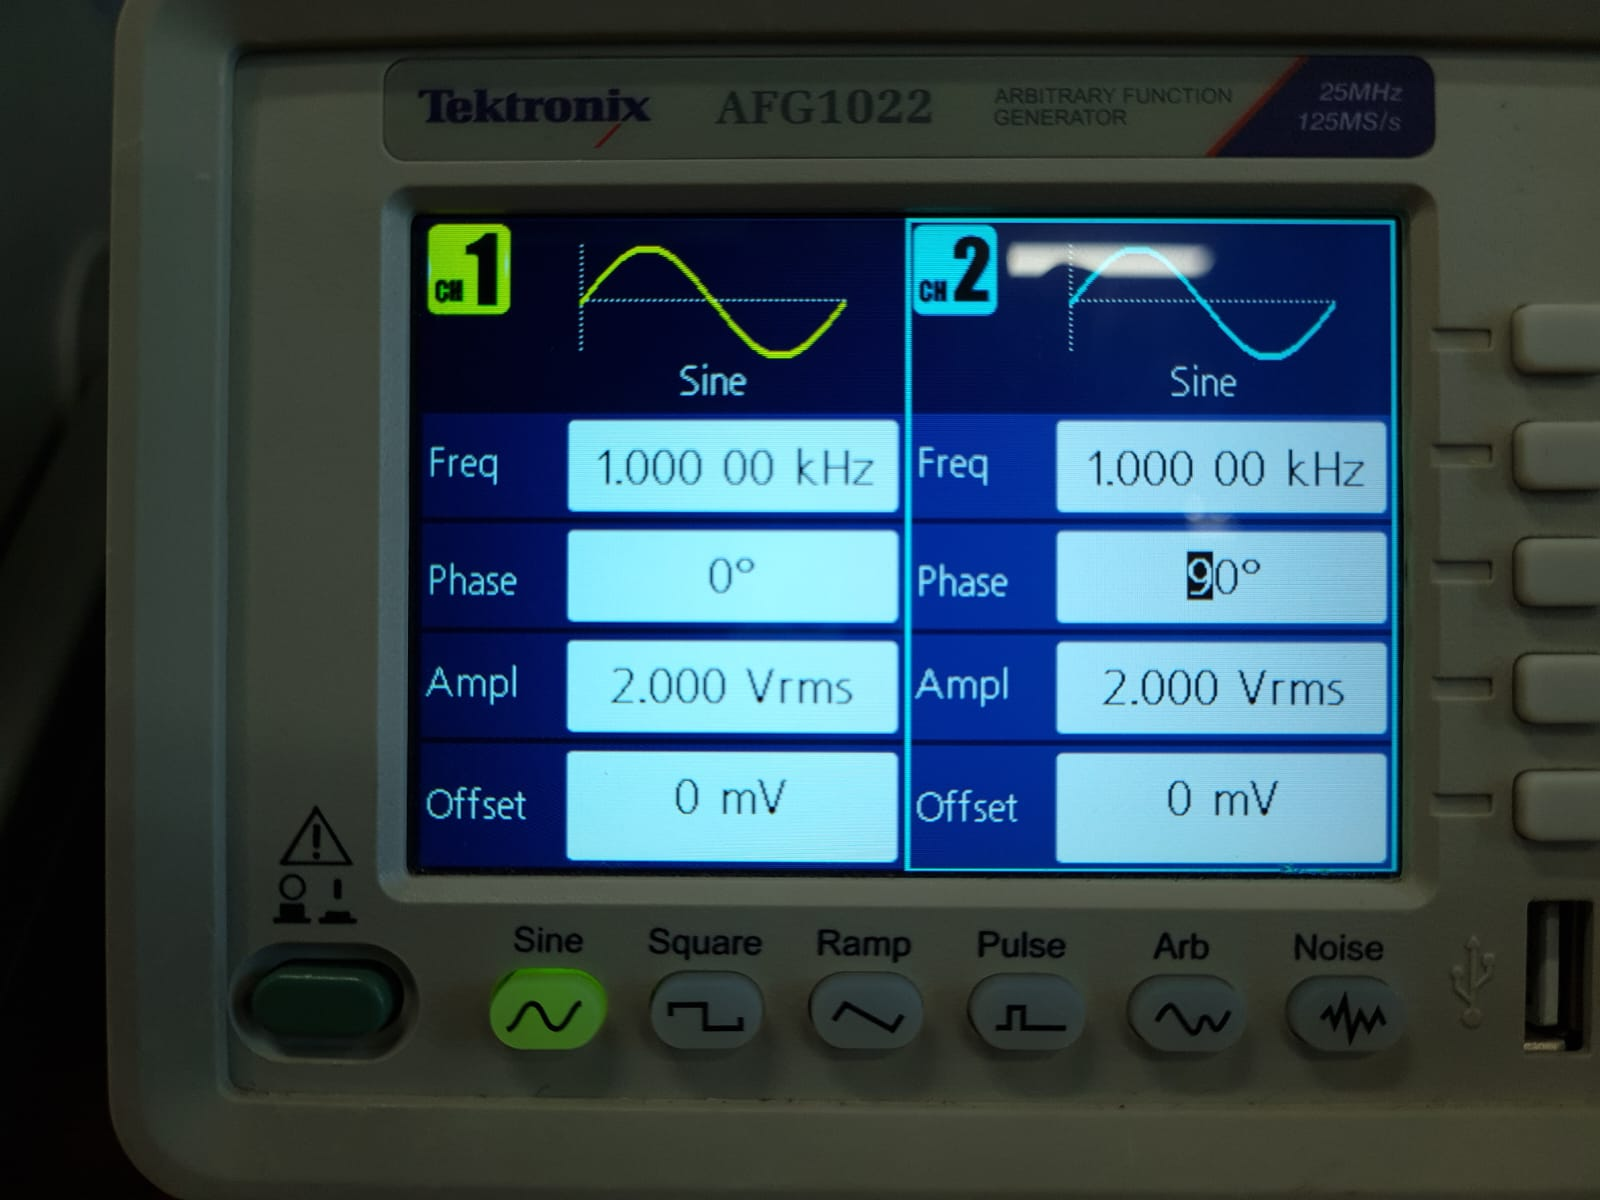
\includegraphics[width=0.5\columnwidth]{/home/gvt1/Work/ECLab2025/experiment01/figs/e2.jpg}\\
		  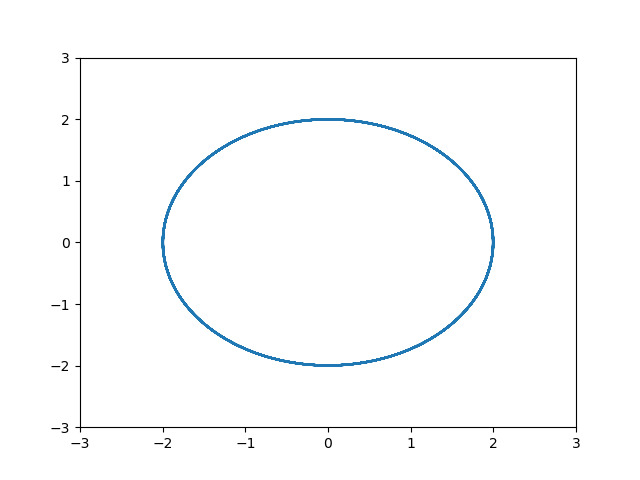
\includegraphics[width=0.4\columnwidth]{/home/gvt1/Work/ECLab2025/experiment01/figs/e.jpg}
		  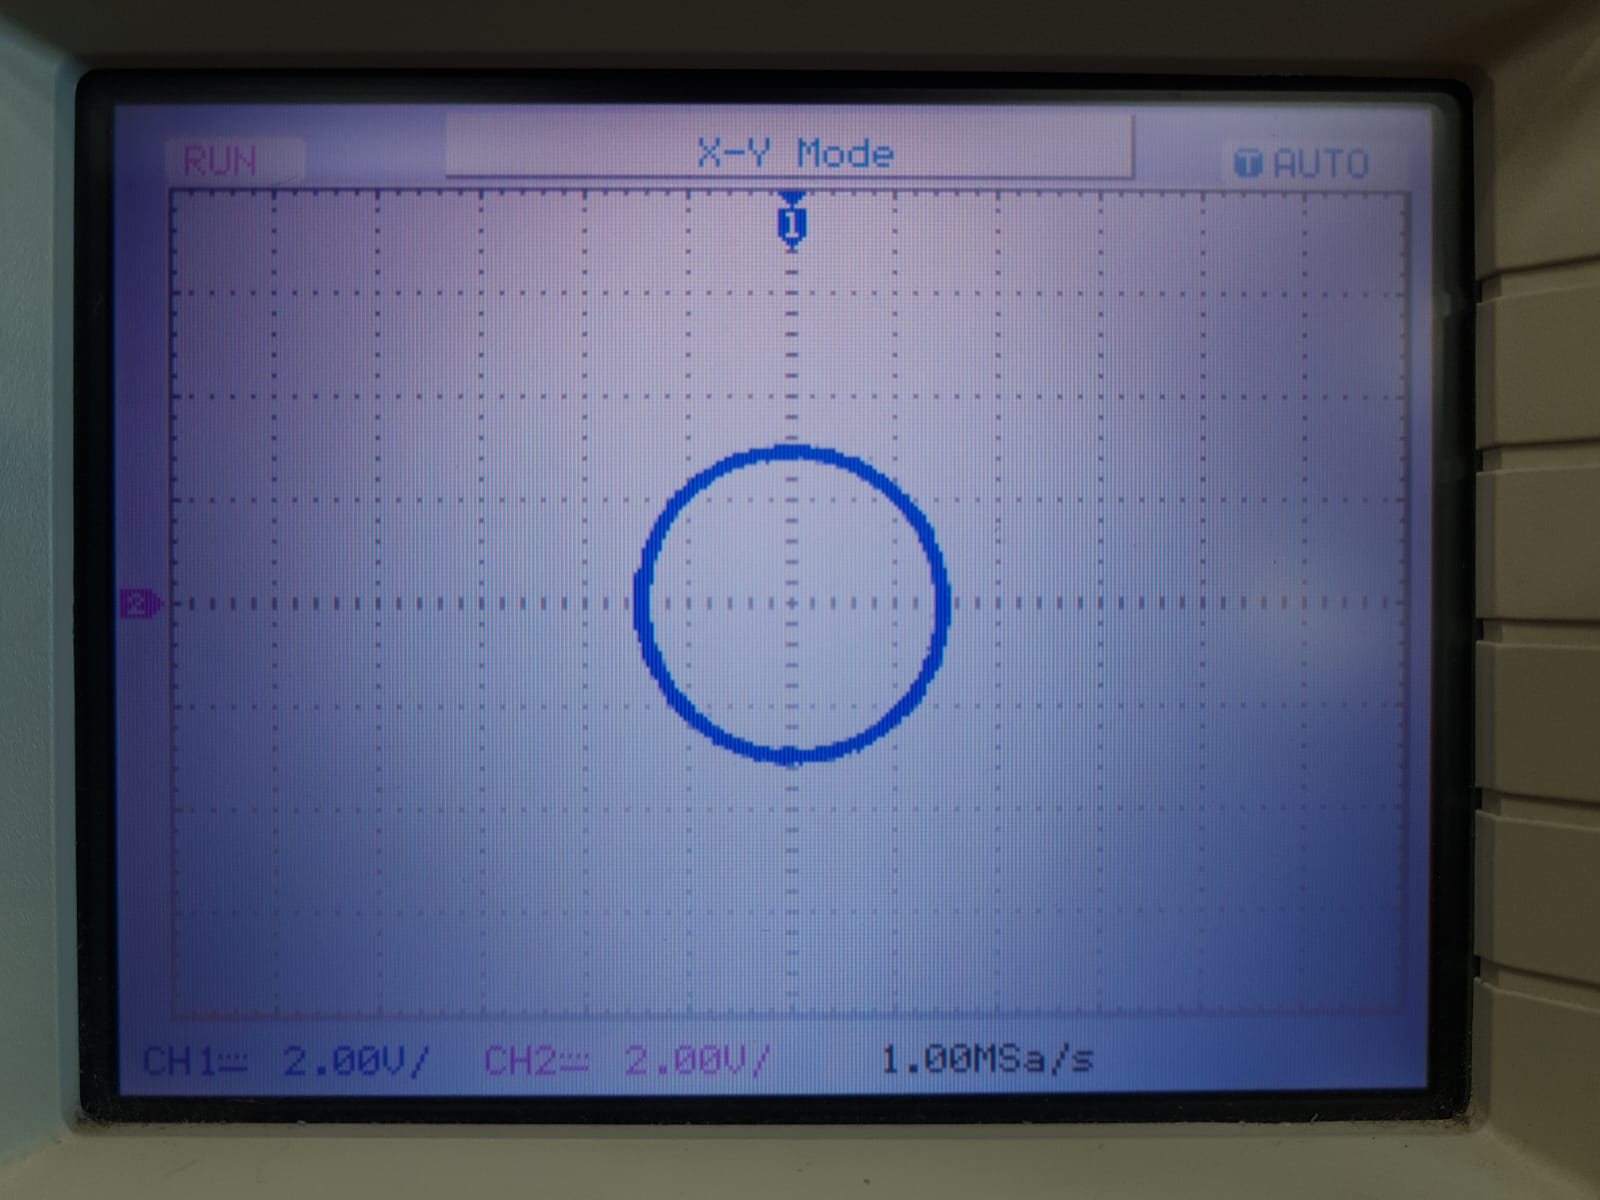
\includegraphics[width=0.4\columnwidth]{/home/gvt1/Work/ECLab2025/experiment01/figs/e1.jpg}\\
		  When the phase difference is $\frac{\pi}{2}$ with all other parameters equal, we end up with a circle because a circle can be paramerterized as $x = a\cos\theta, y = a\sin\theta$, which is how are signals are.
	  \end{center}
\subsection{Conclusion}
We generated simple sinusoidal signals and made Lissajous figures with them, observing patterns emerging from the frequency ratios, symmetry, phase differences; and verified them using code.
\section{Capturing a one-time event on the CRO}
\subsection{Objective}
To capture a one-time event on an oscilloscope, by producing it on a function generator.
\subsection{Apparatus}
\begin{itemize}
	\item Oscilloscope
	\item Function Generator
	\item Connecting probes and wires
\end{itemize}
\subsection{Theory}
An oscilloscope's triggering capability lets us capture a one-time event. Triggering ensures the display starts when the event occurs.\\
Burst mode on the Fuction Generator helps us generate the one-time event.
\subsection{Procedure}
\begin{enumerate}
	\item Set up the oscilloscope and the function generator by connecting the wire and the probe.
	\item Set up the function generator by going to Burst mode, and choosing an appropriate one-time event with a manual trigger.
	\item On the oscilloscope's Mode Coupling settings, ensure that the right channel is being monitored, and the oscilloscope looks for an increasing Edge. Ensure that the Sweep is Normal and the Coupling is DC.
	\item Set an appropriate Trigger level on the oscilloscope.
	\item Select Single mode, the oscilloscope will now start waiting for the one-time event.
	\item Trigger the event on the function generator. Observe on the oscilloscope how we have captured the signal.
\end{enumerate}
\subsection{Demonstration's results}
		\begin{center}
			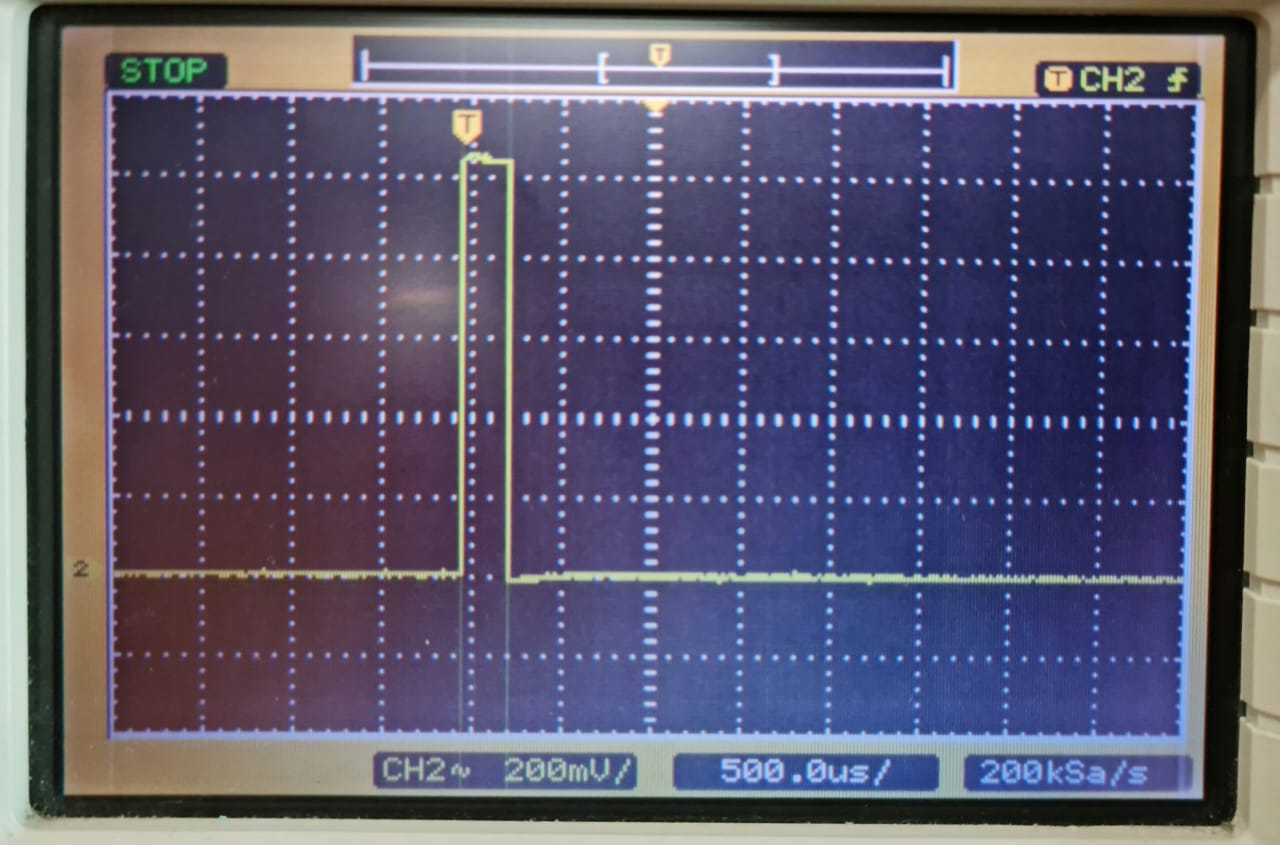
\includegraphics[width=0.7\columnwidth]{/home/gvt1/Work/ECLab2025/experiment01/figs/ote.jpg}\\
			The one-time event we have captured.
		\end{center}
\subsection{Conclusion}
We successfully captured a one-time event. The ability to capture a one-time event on an oscilloscope is of immense value, with numerous applications.
\end{document}
